% !TeX root = skripta-konstitutivni-vztahy.tex
% !TeX lastmodified = 2018-10-30

\section{Model Ogden}
Tento model zavádí energii napjatosti ve tvaru (empirický základ)
\begin{equation}
	W = \sum\limits_{p=1}^N \frac{\mu_p}{\alpha_p} \left(\bar{\lambda}_1^{\alpha_p} + \bar{\lambda}_2^{\alpha_p} + \bar{\lambda}_3^{\alpha_p} - 3\right)
	+ \sum\limits_{p=1}^N \frac{1}{d_p} \left(J - 1\right)^{2p}
\end{equation}
kde:
\begin{description}
	\item[{$\mu_p [\si{\pascal}], \alpha_p [-], d_p [\si{\per\pascal}]$}] jsou materiálové parametry, exponent nemusí být nutně kladný ani celočíselný.
	\item[$\bar{\lambda}_i (i=1,2,3)$] jsou modifikovaná hlavní poměrná protažení, 
	\item[$J$] je třetí invariant tenzoru deformačního gradientu.
\end{description}

Pro $N = 1$ a~$\alpha_p = 2$ dostaneme model Neo-Hooke.

U~obecného Ogdenova modelu je počáteční modul pružnosti ve smyku
\begin{equation}
	G = \frac{1}{2} \sum\limits_{p=1}^N \alpha_p \mu_p
\end{equation}

Pro počáteční objemový modul pružnosti $K$ zde platí vztah
\begin{equation}
	K = \frac{2}{d_1}
\end{equation}

\subsection{OGDENOVA FORMULACE (1972)}
\begin{itemize}
	\item Poprvé po 30 letech upustil od používání Mooney-Rivlinova formalismu.
	\item Zřejmě navázal na myšlenku Valanise a Lendela (1967), kteří navrhli modelovat $W$ přímo jako funkci hlavních protažení:
	\begin{equation}
		W = w(\lambda_1) + w(\lambda_2) + w(\lambda_3)
	\end{equation}
	\item Původně formulován jako nestlačitelný.
	\item Spolehlivě funguje i~pro extrémně velké deformace.
	\item $\mu_p$, $\alpha_p$ mohou být kladná i~záporná reálná čísla
	\item Skvělá predikční schopnost pro
	\begin{itemize}
		\item jednoosý tah (až do 700\% deformace)
		\item ekvibiax
		\item prostý smyk
	\end{itemize}
\end{itemize}

\begin{figure}[H]
	\centering
	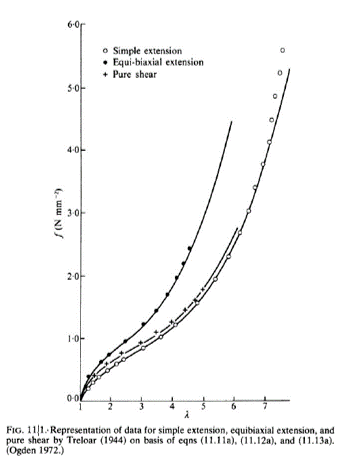
\includegraphics[height=5cm]{ogden}
	\caption{Aproximace experimentu Ogdenovým modelem}
	\label{fig:ogden}
\end{figure}
